\documentclass[12pt]{article}
\usepackage[scaled]{helvet}
\renewcommand\familydefault{\sfdefault} 
\usepackage[T1]{fontenc}

\usepackage[english]{babel}
\usepackage[utf8]{inputenc}
\usepackage{amsmath}
\usepackage{bm}
\usepackage{parskip}
\usepackage{hyperref}
\usepackage{graphicx}
\usepackage{listings}
\usepackage{xcolor}

\definecolor{Brown}{cmyk}{0,0.81,1,0.60}
\definecolor{OliveGreen}{cmyk}{0.64,0,0.95,0.40}
\definecolor{CadetBlue}{cmyk}{0.62,0.57,0.23,0}
\definecolor{lightlightgray}{gray}{0.9}

\lstset { %
    language=C++,
    %backgroundcolor=\color{black!5}, % set backgroundcolor
    %basicstyle=\footnotesize,% basic font setting
	basicstyle=\ttfamily,                   % Code font, Examples: \footnotesize, \ttfamily
	keywordstyle=\color{OliveGreen},        % Keywords font ('*' = uppercase)
	commentstyle=\color{gray},              % Comments font
	backgroundcolor=\color{lightlightgray},
	tabsize=4,
	frame=single,
}

\title{\textbf{Practical 8: Rigid Bodies, part 3 }}
\author{Babis Koniaris}
\date{}

\begin{document}
\maketitle

\begin{center}
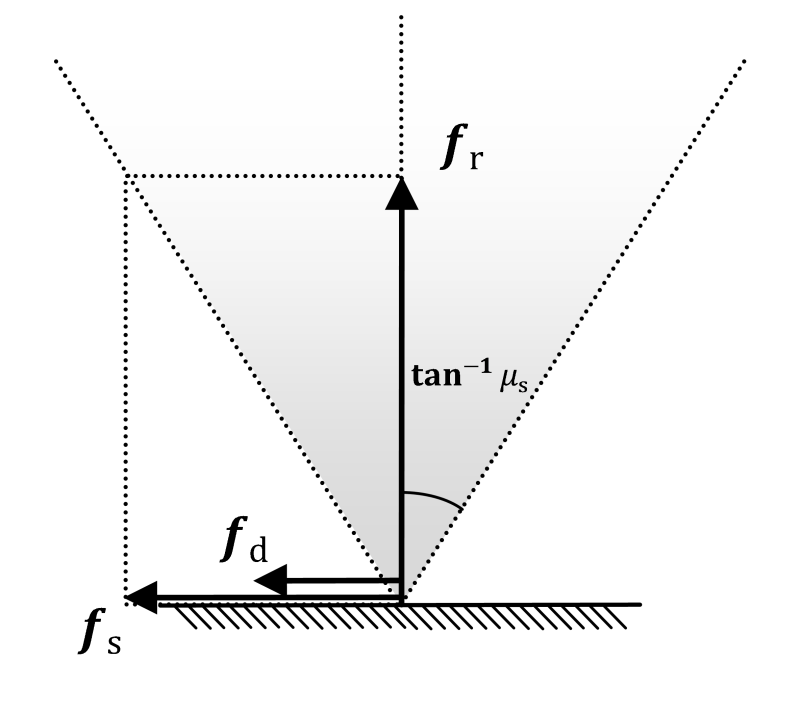
\includegraphics[width=\textwidth]{p8-teaser.png}
\end{center}
\pagebreak

\section*{Introduction}

The goal of this practical is to deliver a working rigid body simulation that includes the
following features:

\begin{itemize}
\item Works for a solid cuboid
\item Collision detection with a horizontal plane
\item Impulse-based collision response
\item Simulates friction with a horizontal plane
\end{itemize}

\section*{Tasks}

\subsection*{Task 1: Application of an impulse}

For this task and all subsequent tasks, create a default cubic rigid body scale it by a
factor of \textbf{3 along the y axis}. You will end up with a cuboid that has a width of 2, a height of
6 and a depth of 2. Assign a \textbf{mass of 2} to it.

\begin{itemize}
\item Output the inverse inertia matrix of the rigid body on the console \footnote{Note that you can display any glm object as a string using glm::to\_string, which is part of the glm/ext.hpp library}
\item Assign an initial velocity of (2,0,0) and initial angular velocity of (0,0,0) to the solid. Do not assign any force to it. After 2 seconds, apply a single impulse to the solid so that its center of mass comes to a stop and the solid starts spinning clockwise. 
\end{itemize}

\subsection*{Task 2: Collision detection}

\textbf{Task 2: Detect which vertex or vertices of a cuboid collide with the ground plane}

To demonstrate your solution, output the following information to the console when a collision is detected:
\begin{itemize}
\item Coordinates of all colliding vertices \footnote{1 if the collision is with a vertex, 2 if it’s with an edge and 4 if it’s with a face}
\item Average of all colliding coordinates \footnote{Hopefully you will have figured out in last week’s practical that this information is mandatory to implement the collision response!}
\end{itemize}

\subsection*{Task 3: Collision response}

\textbf{Task 3: Simulate the collision between a rigid body (cuboid) and the ground plane using impulse-based collision response}

Here are the specific simulations you will demonstrate:

\begin{itemize}
\item Assign an angular velocity of (0,0,0.5) to the solid and an elasticity of 1 \footnote{this refers to the elasticity value used in the collision response impulse}
\item Assign an angular velocity of (0.1,0.1,0.1) to the solid and an elasticity of 0.7
\end{itemize}

You are welcome to demonstrate other cases too.

\subsection*{Task 4: Friction}

\textbf{Task 4: Add a model of friction to your simulation and any other operations of your own design that will make the solid stop in a realistic fashion.}

The focus of this task should be to achieve a realistic simulation for an elasticity of around 0.6. You should aim to make the solid stop translating and rotating realistically. Use the theory \emph{liberally} and \emph{creatively} to achieve your goal.

\section*{Deliverables}

\subsection*{Marking scheme}

Here's a summary of what you need to deliver and allocated marks:
\begin{itemize}
\item \textbf{Task 1: Impulse application: 5 marks}
\item \textbf{Task 2: Collision detection: 6 marks}
\item \textbf{Task 3: Collision response (no friction): 9 marks}
\item \textbf{Task 4: Collision response (w/ friction): 5 marks}
\end{itemize}

\subsection*{Submission details}

You must submit your work using the relevant Moodle assignment by the deadline specified on Moodle. Please submit your zipped code and executable.

\end{document}